\renewcommand*{\thefootnote}{\fnsymbol{footnote}}
\def\equalfootnote{\mathrel{\ensurestackMath{\stackon[0.5pt]{=}{\footnotemark[2]}}}}

\makeatletter
\newcommand{\smallbullet}{} % for safety
\DeclareRobustCommand\smallbullet{%
  \mathord{\mathpalette\smallbullet@{0.75}}%
}
\newcommand{\smallbullet@}[2]{%
  \vcenter{\hbox{\scalebox{#2}{$\m@th#1\bullet$}}}%
}
\makeatother
%//==============================--@--==============================//%
\subsection[2.2 Modelação de Sistemas Físicos]{\hspace*{0.075 em}\raisebox{0.2 em}{$\pmb{\drsh}$} Modelação de Sistemas Físicos}
\label{sec:mechanics}
%//==============================--@--==============================//%
\subsubsection[2.2.1 Sistemas Mecânicos de Translação]{$\pmb{\rightarrow}$ Sistemas Mecânicos de Translação}
\label{sec:mechanics-translation}

\begin{quote}
    ``The cornerstone for obtaining a mathematical model, or the dynamic equations, for any mechanical system is Newton's law
    $$
        \boxed{F = \frac{dp}{dt} = \frac{d}{dt} (m v) \equalfootnote ma}
    $$
    \noindent where:
    \begin{itemize}[leftmargin=*,label=${\smallbullet}$]
        \item $F$ = the vector sum of all forces applied to each body in a system, newtons (N),
        \item $p$ = linear momentum/translational momentum (kg ms$^{-1}$),
        \item $v$ = velocity (ms$^{-1}$), the directional speed of an object in motion as an indication of its rate of change in position as observed from a particular frame of reference,
        \item $a$ = the vector acceleration of each body with respect to an inertial reference frame (that is, one that is neither accelerating nor rotating with respect to the stars); often called inertial acceleration, ms$^{-2}$,
        \item $m$ = mass of the body, kg.''\cite{FranklinPowell2015}
    \end{itemize}
\end{quote}

\footnotetext[2]{Para uma massa invariante no tempo, ou aproximadamente constante.}
\renewcommand*{\thefootnote}{\arabic{footnote}}

\phantomsection\addcontentsline{toc}{subsubsection}{3.1.1 Relações fundamentais baseadas em princípios físicos}
\renewcommand*{\thefootnote}{\fnsymbol{footnote}}
\begin{theo}[\underline{Molas Elásticas}]{def:Molas Elásticas}\label{def:MolasElásticas}
Quando uma mola é comprimida ou esticada, reage com uma força que se opõe à compressão (ou à extensão). Força desta que, para molas lineares, é dada por:
$$
    f = -kx
$$
Onde $k$ é a constante de Hooke [N/m].
\end{theo}

\begin{theo}[\underline{Atrito Viscoso}]{def:Atrito Viscoso}\label{def:AtritoViscoso}
Elemento que dissipa energia. Quando existe uma diferença de velocidade entre dois corpos o atrito corresponde a uma força que contraria o movimento. No caso linear, o atrito é dado por:
$$
    f = -\beta\dot{x}\ = -\beta v 
$$
\end{theo}

%//==============================--@--==============================//%
\subsubsection[2.2.2 Sistemas Mecânicos de Rotação]{$\pmb{\rightarrow}$ Sistemas Mecânicos de Rotação}
\label{sec:mechanics-rotation}

O \underline{Momento de Inércia} é o análogo da massa para a rotação. Quando um corpo em rotação com um \underline{Momento de Inércia} $J$ $[$Nms$^{2}]$ é atuado por um \underline{Binário} $T$ $[$Nm$]$, adquire aceleração angular dada por
$$
    \boxed{J\ddot{\theta} = T}
$$

\vspace{-1em}
\begin{theo}[\underline{Molas Elásticas}]{def:Mola Elástica de Rota}\label{def:MolaElasticaRota}
Quando a mola é desviada um ângulo $\theta$  em relação à posição de repouso, reage
com um binário que se opõe ao movimento, dada para molas lineares por:
$$
    T = -K\dot{\theta}\ 
$$
Onde $k$ é a "constante da mola" [Nm/rads$^{-1}$].
\end{theo}

\begin{theo}[\underline{Atrito Viscoso}]{def:Atrito Viscoso Rotação}\label{def:AtritoViscosoRotação}
Elemento que dissipa energia. Quando existe uma diferença de velocidade de rotação entre dois corpos o atrito corresponde a uma binário que contraria o movimento e que depende da velocidade angular. No caso linear, o atrito é dado por:
$$
    T = -\beta\dot{\theta}\ = -\beta \omega
$$
\end{theo}

\begin{theo}[\underline{Transformação da rotação em translação}]{def:rotation-to-translation}\label{def:rotation-to-translation}
Assumindo que não existe escorregamento, nem perdas energéticas, temos:
\begin{figure}[H]
    \centering
    \begin{minipage}{0.6\linewidth}
        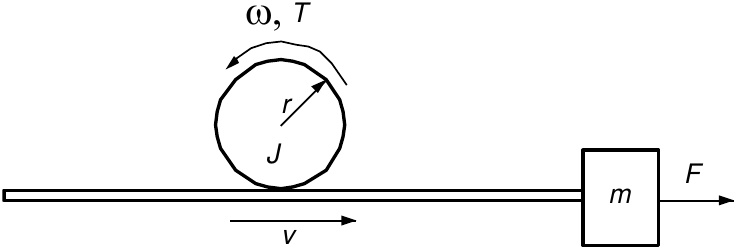
\includegraphics[width = 1\linewidth]{img/1/convertion.png} \label{fig:convertion}
    \end{minipage}
    \hfill
    \raisebox{0.75em}{\begin{minipage}{0.33\linewidth}\resizebox{0.55\hsize}{!}{$%
        \left\{
        \begin{aligned}
            v &= \omega r \\ 
            F &= \frac{1}{r} T
        \end{aligned}
        \right.
    $}
    \end{minipage}}
\end{figure}
\end{theo}

%//==============================--@--==============================//%
\newpage
\subsubsection[2.2.3 Motor Corrente Contínua]{$\pmb{\rightarrow}$ Motor de Corrente Contínua}
\mdfsetup{linewidth=2pt}
\begin{mdframed}
\textbf{Modelo do servomotor CC de íman permanente:}

\noindent\underline{Binário do motor}: Para um fluxo constante

\noindent \hspace*{1.5 em}\raisebox{0.2 em}{$\drsh$} $T(t) = K_T\, i(t)$

\vspace{0.5em}
\noindent\underline{Tensão aos terminais do rotor}: 

\noindent \hspace*{1.5 em}\raisebox{0.2 em}{$\drsh$} $e = K_e\, \omega$
%adoro-te :3 miminhooooooooooooooooooooooooooooooooooooooos

% cutie :3 -><- aaaaaaadoro-te
\end{mdframed}
\paragraph[2.2.3.1 Problema 1]{$\pmb{\star}$ Escreva as equações que modelam o sistema na forma de um modelo de estado (sistema
de equações diferenciais de 1ª ordem)}\mbox{}\\
\begin{figure}[H]
    \centering
    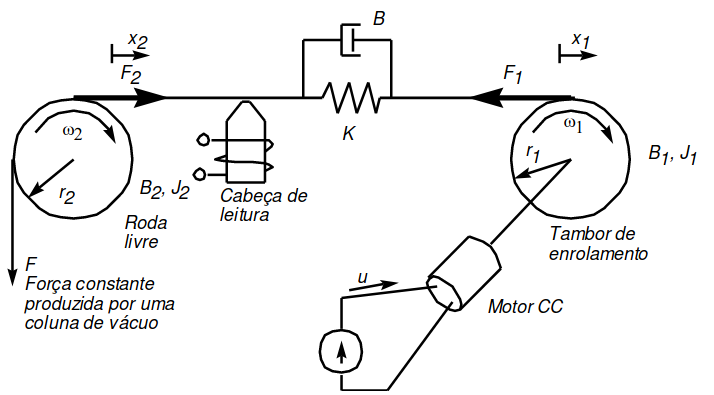
\includegraphics[width = 0.6\linewidth]{img/1/motor-cc-P16.png}
    \caption{P16 retirado da coletânea de exercícios.}
    \label{fig:motor-cc-P16}
\end{figure}

\noindent\underline{T. de Enrolamento}: de acordo com as equações subjacentes à mecânica de rotação

\noindent \hspace*{1.5 em}\raisebox{0.2 em}{$\drsh$} $J_1 \dot{\omega_1} = - F_1 r_1 - \beta_1 \omega_1 + T_{cc}$

\vspace{0.5em}
\noindent\underline{Roda Livre}: novamente, de acordo com as equações subjacentes à mecânica de rotação 

\noindent \hspace*{1.5 em}\raisebox{0.2 em}{$\drsh$} $J_1 \dot{\omega_2} = (F_2 - F) r_2 - \beta_2 \omega_2$

\vspace{0.5em}
\noindent\underline{Fita}: (\textit{vide} \hyperref[def:MolasElásticas]{secção das molas elásticas})

\noindent \hspace*{1.5 em}\raisebox{0.2 em}{$\drsh$} $
                \begin{cases}
                    F_1 = K(x_1 - x_2) + \beta(\dot{x_1} - \dot{x_2})\\
                    F_2 = -K(x_2 - x_1) - \beta(\dot{x_2} - \dot{x_1})\\
                \end{cases}
$

\vspace{0.5em}
\noindent\underline{Motor CC}: $T_{cc}$ é o binário exercido pelo motor CC no Tambor de Enrolamento

\noindent \hspace*{1.5 em}\raisebox{0.2 em}{$\drsh$} $T_{cc} = K_T\, u$

\vspace{0.5em}
\noindent\underline{Variáveis do referencial}: a velocidade linear de um ponto da periferia de uma roda é o produto do raio da roda pela velocidade angular

\noindent \hspace*{1.5 em}\raisebox{0.2 em}{$\drsh$} $
                \begin{cases}
                    \dot{x_1} = \omega_1 r_1\\
                    \dot{x_2} = \omega_2 r_2\\
                \end{cases}
$

%//==============================--@--==============================//%
\clearpage
\paragraph[2.2.3.2 Problema 2]{$\pmb{\star}$ Escreva as equações que modelam o sistema e um modelo de estado na forma de um sistema de
equações diferenciais de 1ª ordem.}\mbox{}\\
\begin{figure}[H]
    \centering
    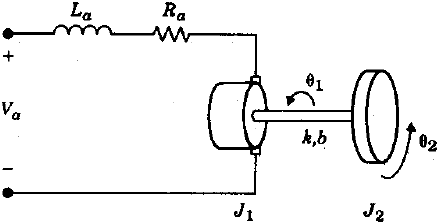
\includegraphics[width = 0.45\linewidth]{img/1/motor-cc-P18.png}
    \caption{P18 retirado da coletânea de exercícios. Motor elétrico que reboca uma carga com um modo dominante de vibração.}
    \label{fig:motor-cc-P18}
\end{figure}

\noindent \underline{Motor:} por aplicação da Lei das Malhas (KVL)

\noindent \hspace*{1.5 em}\raisebox{0.2 em}{$\drsh$} \textbf{KVL:} $ L_a \dfrac{d i_a}{dt} + i_a R_a + e_a - V_A = 0 \iff \dfrac{d i_a}{dt} = -\dfrac{K_e}{L_a} \dot{\theta}_1 - \dfrac{R_a}{L_a} i_a + V_A$

\vspace{0.5em}
\noindent \underline{Veio:} com as equações subjacentes à mecânica de rotação

\noindent \hspace*{1.5 em}\raisebox{0.2 em}{$\drsh$} $J_1 \ddot{\theta}_1 = -K(\theta_1 - \theta_2) -\beta(\dot{\theta}_1 - \dot{\theta}_2) + T_{cc}$

\vspace{0.5em}
\noindent\underline{Motor CC}: $T_{cc}$ é o binário exercido pelo motor CC no veio

\noindent \hspace*{1.5 em}\raisebox{0.2 em}{$\drsh$} $T_{cc} = K_T\, i_a$

\vspace{0.5em}
\noindent \underline{Carga:} de acordo com as equações subjacentes à mecânica de rotação

\noindent \hspace*{1.5 em}\raisebox{0.2 em}{$\drsh$} $J_2 \ddot{\theta}_2 = -K(\theta_2 - \theta_1) -\beta(\dot{\theta}_2 - \dot{\theta}_1)$

\vspace{0.5em}
\noindent Definem-se então os estados: $\pmb{x} = \begin{bmatrix} \theta_2 & \dot{\theta}_2 & \theta_1 & \dot{\theta}_1 & i_a\end{bmatrix}^T$

$$
    \therefore \dot{\pmb{x}} = 
    \begin{bmatrix} 
        0 & 1 & 0 & 0 & 0\\[4pt]
        -\frac{K}{J_2} & -\frac{\beta}{J_2} & \frac{K}{J_2} & \frac{\beta}{J_2} & 0\\[4pt]
        0 & 0 & 0 & 1 & 0\\[4pt]
        \frac{K}{J_1} & \frac{\beta}{J_1} & -\frac{K}{J_1} & -\frac{\beta}{J_1} & K_T\\[4pt]
        0 & 0 & 0 & -\frac{K_e}{L_a} & -\frac{R_a}{L_a}
    \end{bmatrix}
    \pmb{x} +
    \begin{bmatrix} 
        0\\
        0\\
        0\\
        0\\
        -\frac{1}{L_a}
    \end{bmatrix}
    V_A
$$

%//==============================--@--==============================//%
\clearpage
\paragraph[2.2.3.3 Problema 3]{$\pmb{\star}$ Defina um estado apropriado com a menor dimensão possível e escreva as respetivas equações de estado na forma matricial.}\mbox{}\\
\begin{figure}[H]
    \centering
    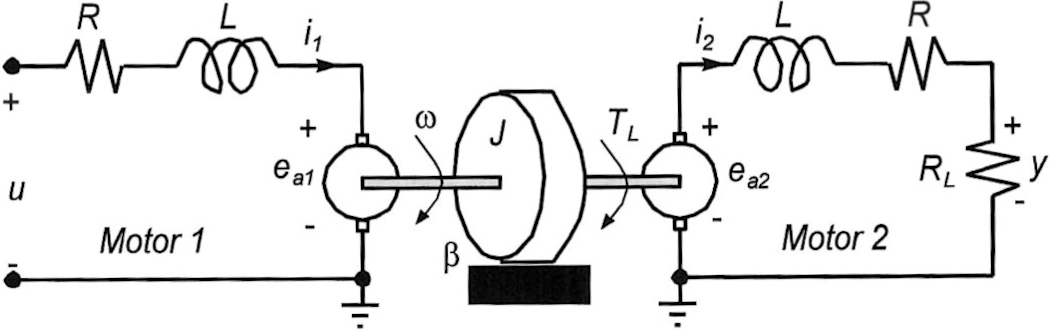
\includegraphics[width = 0.6\linewidth]{img/1/motor-cc-exame2021.png}
    \caption{Circuito eletromecânico equivalente de dois motores de corrente contínua de íman permanente, que têm os veios ligados solidariamente. $T_L = K_T\, i_1$ e $e_{ai} = K_{ei}\, \omega$}
    \label{fig:motor-cc-exame20/21}
\end{figure}

\noindent \underline{Motor 1:} por aplicação da Lei das Malhas (KVL)

\noindent \hspace*{1.5 em}\raisebox{0.2 em}{$\drsh$} \textbf{KVL:} $i_1 R + L \dfrac{d i_1}{dt} + e_{a1} - u = 0 \iff \dfrac{d i_1}{dt} = - \dfrac{R}{L} i_1 - \dfrac{K_{e1}}{L} \omega + \dfrac{1}{L}u$

\vspace{0.5em}
\noindent \underline{Motor 2:} por aplicação, novamente, da Lei das Malhas (KVL)

\noindent \hspace*{1.5 em}\raisebox{0.2 em}{$\drsh$} \textbf{KVL:} $L \dfrac{d i_2}{dt} + i_2 R + i_2 R_L - e_{a2} = 0 \iff \dfrac{d i_2}{dt} = \dfrac{K_{e2}}{L}\omega - \left(\dfrac{R+R_L}{L}\right) i_2$

\vspace{0.5em}
\noindent \underline{Roda:} de acordo com as equações subjacentes à mecânica de rotação

\noindent \hspace*{1.5 em}\raisebox{0.2 em}{$\drsh$} $J \dot{\omega} = T_L - \beta \omega \iff \dot{\omega} = -\dfrac{\beta}{J}\omega + \dfrac{K_T}{J} i_1$

\vspace{0.5em}
\noindent Definem-se então os estados: $\pmb{x} = \begin{bmatrix} \omega & i_1 & i_2 \end{bmatrix}^T$

$$
    \therefore \dot{\pmb{x}} = 
    \begin{bmatrix} 
        -\frac{\beta}{J} & \frac{K_T}{J} & 0\\[5pt]
        -\frac{K_{e1}}{L} & -\frac{R}{L} & 0\\[5pt]
        \frac{K_{e2}}{L} & 0 & \frac{K_T}{J}
    \end{bmatrix}
    \pmb{x} +
    \begin{bmatrix} 
        0\\[5pt]
        \frac{1}{L}\\[5pt]
        0
    \end{bmatrix}
    u,\qquad y = 
    \begin{bmatrix}
        0 & 0 & R_L
    \end{bmatrix}
    \pmb{x}
$$

%//==============================--@--==============================//%